\documentclass[12pt]{article}
\usepackage{amsmath}
\usepackage{graphicx}
\begin{document}
\newtheorem{definition}{Definition}
\newtheorem{theorem}{Theorem}
\newtheorem{example}{Example}

\section{Buildings}
\begin{definition}
  A Polyhedral complex is a certain finite dimensional CW-complex. Each n-cell of the polyhedral complex is   
\end{definition}

\begin{definition}
    Suppose P is a simple convex polytope in $X^n$. Let $F_i$ be the codimension-one faces of P. Suppose that, for any two faces Fi and Fj, if their intersection is non-empty, then the dihedral angle between the faces is pi/mij, for some mij in ${2,3,4,...}$. Now set $mii=1, mij=inf$ if Fi, Fj empty intersection. Let $s_i$ be the reflection of $X^n$ across Fi, and let W be the group generated by the set of si's. Then W is the Coxeter group with generators $s_i$, and Coxeter matrix $(mij)$. Furthermore, W is a discrete subgroup of Isom($X^n$), P is a strict fundamental domain for the W action, and P tiles $X^n$. 
\end{definition}   
    
\begin{definition}
    Let $(W,S)$ be a Coxeter group generated by a simple convex polytope P. A building of type $(W,S)$ is a polyhedral complex, which is a union of subcomplexs, called apartments. An apartment is isometric to the tiling of $X^n$ derived from P, and each copy of P in the tiling is called a chamber. Now the apartments and chambers must satisfy
    \begin{enumerate}
    \item Given any two chambers, there exists an aprtment containing both of them.
    \item Given any two apartments A and B, there exists an isometry from A to B which fixes $A \cap B$ pointwise. 
    \end{enumerate}
\end{definition}

\begin{example}
    Let us consider a single copy of $X^n$. We can tile this copy by P, and we get a thin building. This means that we only have one apartment. Clearly this satisfies the first condition - any two chambers immediately lie in the only apartment. 

    Now let us look at the second condition. If the two chambers have no intersection, then, as each chamber is a copy of P, they are clearly isometric, and we are done. Now if the two chambers have a non-empty intersection, we have two cases:
    \begin{enumerate}
        \item If they share a common edge, then reflection along this edge gives us our isometry.
        \item If they only share a common point
    \end{enumerate}
\end{example}

\begin{example}
    Now we can consider a spherical building. Take the Coxeter group
    \[W=\langle s_1,s_2 | s_i^2=1, (s_1s_2)^2=1\rangle.
    \]
    This Coxeter group is isomorphic to $D_4$. 
\end{example}

\section{Cayley graphs}
\begin{definition}
    The Cayley graph Cay(G,S) of a group $G$ with respect to a generating set $S$, $1\notin S$, is the graph $(V,E)$, with $V=G$, and directed edges
    \[E=\{(g,gs)|g\in G, s\in S\}.\]
    If $s\in S$ is an involution, we only put a single undirected edge between $g$ and $gs$, and label the edge $s$. 
\end{definition}

\begin{example}
    The Cayley graph of $D_6$, with generating set $\{s_1,s_2\}$ is 


    \centering{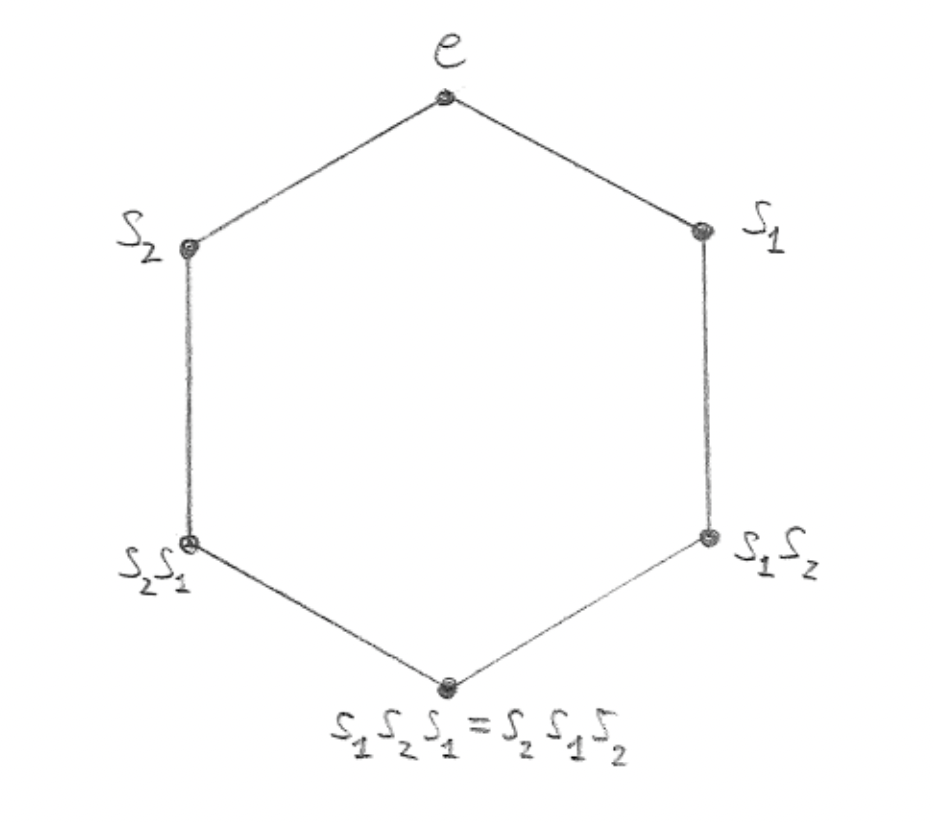
\includegraphics[scale=0.4]{Screenshot 2023-01-03 at 12.40.32.png}}
\end{example}
\section{Reflection systems}
\begin{definition}
    Let $G$ be a group. A pre-reflection system for $G$ is a pair $(X,R)$. $X$ is a connected simplicial graph which is acted upon by $G$, and $R$ is a subset of $G$. This must satisfy
    \begin{enumerate}
        \item every element of $R$ is an involution;
        \item R is closed under conjugation;
        \item R generates G;
        \item given an edge of $X$, there is a unique element of $R$ which flips the edge; and
        \item for every element $r$ of $R$, there is at least one edge of $X$ which is flipped by $r$. 
    \end{enumerate}
\end{definition}

\begin{example}
    Let $(W,S)$ be any Coxeter system. Let $X$ be the Cayley graph of $(W,S)$, and let
    \[ R=\{wsw^{-1}|w\in W, s\in S\}. \]
    Then $(X,R)$ is a pre-reflection system.
\end{example}

\begin{definition}
    Consider a pre-reflection system $(X,R)$. For each element $r$ of $R$, the wall $H_r$ is the set of midpoints of all the edges flipped by $r$. 
\end{definition}

\begin{definition}
    Consider a pre-reflection system $(X,R)$. If, additionally, it satisfies
    \begin{enumerate}
        \setcounter{enumi}{5}
        \item for every element $r$ in $R$, $X\backslash H_r$ has exactly two components,
    \end{enumerate}
    then $(X,R)$ is a reflection system. 
\end{definition}


\begin{theorem}
    Suppose we have a group $W$, generated by a set $S$ of distinct involutions. Then the following are equivalent:
    \begin{enumerate}
        \item $(W,S)$ is a Coxeter system;
        \item $(X,R)$ is a reflection system, where $X=Cay(W,S)$ and \[R=\{wsw^{-1}|w\in W, s\in S\}.\]
        \item $(W,S)$ satisfies the Deletion Condition; and
        \item $(W,S)$ satisfies the Exchange Condition.
    \end{enumerate}
\end{theorem}


\section{Tits' solution to the word problem}

\begin{definition}
    Let $W$ be generated by a set $S$ of distinct involutions. Let $s,t\in S$, with $s\neq t$, and let $m_{st}$ be the order of $st$ in $W$. If $m_{st}$ is finite, consider a word in $S$ with the subword $sts...$ with $m_{st}$ letters. A braid move on the word replaces the subword $sts...$ with $tst...$, again with $m_{st}$ letters. 
\end{definition}

\begin{theorem}
    (Tits) Suppose we have a group $W$, generated by a set $S$ of distinct involutions. Also suppose that the Exchange Condition holds. Then
    \begin{enumerate}
        \item A word $s_1s_2...s_k$ is reduced iff we cannot shorten it by a sequence of 
        \begin{itemize}
            \item deleting an instance of $ss$ from the word, or
            \item applying a braid move to the word.
        \end{itemize}
        \item Two reduced words will represent the same group element iff a sequence of braid moves sends one to the other.
    \end{enumerate}
\end{theorem}




























\end{document}

